\documentclass[a4paper,12pt]{report}
\usepackage[utf8]{inputenc}
\usepackage[T1]{fontenc}
\usepackage[french]{babel}
\usepackage{graphicx}
\usepackage{geometry}
\usepackage{setspace}
\usepackage{hyperref}
\usepackage{float}

\geometry{margin=2.5cm}
\setstretch{1.5}
\graphicspath{{figures/}}

% ============================================================
%  INFORMATIONS PERSONNELLES -- A REMPLIR PAR L'ETUDIANT(E)
%  (le PDF fourni contient des placeholders visibles TODO-*)
% ============================================================
\newcommand{\EtudiantNom}{TODO-NOM Pr\'enom}            % ex. \textsc{Ayari Farah}
\newcommand{\EcoleNom}{\'Ecole sup\'erieure priv\'ee d'ing\'enierie et de technologie}
\newcommand{\EntrepriseNom}{TODO-SOCIETE}               % ex. societe
\newcommand{\EncadrantNom}{TODO-NOM-ENCADRANT}          % ex. nom
\newcommand{\StagePeriode}{TODO-DATES}                  % ex. Du 5 juillet au 20 ao\^ut 2025
\newcommand{\AnneeUniv}{2025 -- 2026}
\newcommand{\SujetStage}{Conception et \'evaluation d'un syst\`eme de question-r\'eponse documentaire multilingue (RAG) appliqu\'e \`a des documents bancaires}

\begin{document}

% ======================
% PAGE DE GARDE
\begin{titlepage}
\noindent
\begin{minipage}[t]{0.2\textwidth}
    \IfFileExists{esprit.png}{\includegraphics[width=3.5cm]{esprit.png}}{%
    \fbox{\parbox[c][2.2cm][c]{3.2cm}{\centering \small Logo \'ecole}}}
\end{minipage}
\hfill
\begin{minipage}[t]{0.75\textwidth}
    \centering
    \textbf{\large R\'epublique Tunisienne} \\[0.2cm]
    \textbf{\large \EcoleNom}
\end{minipage}

\vspace{2cm}

\begin{center}
\Huge \textbf{Rapport de Stage d'Immersion en Entreprise} \\
\vspace{1.5cm}
\Large Sujet : \textbf{\SujetStage} \\
\vspace{1.5cm}
\Large R\'ealis\'e au sein de \textbf{\EntrepriseNom} \\
\vspace{1.5cm}
\textbf{\StagePeriode} \\
\vspace{1cm}
\textbf{\'Elabor\'e par} \textsc{\EtudiantNom} \\
\vspace{0.5cm}
\textbf{Encadr\'e par} \textsc{\EncadrantNom} \\
\vspace{0.5cm}
\textbf{Ann\'ee universitaire \AnneeUniv}
\end{center}
\end{titlepage}

% ======================
% TABLE DES MATIERES
\tableofcontents
\listoffigures
\listoftables
\newpage

% ======================
% DEDICACES
\chapter*{D\'edicaces}
\addcontentsline{toc}{chapter}{D\'edicaces}
J'ai le plaisir de d\'edier ce travail \`a :
\begin{itemize}
    \item Mes tr\`es chers parents, pour leur amour, leur patience et leurs encouragements sans faille.
    \item Mes s\oe urs et mon fr\`ere, pour leur soutien et leur pr\'esence rassurante.
    \item Mes amis proches qui ont toujours \'{e}t\'e l\`a pour me soutenir dans ce parcours.
    \item Mes grands-parents, dont les pri\`eres m'accompagnent chaque jour.
    \item Mes oncles et tantes qui m'ont toujours soutenue, chacun \`a sa mani\`ere.
    \item Tous mes collaborateurs et coll\`egues de stage pour leur soutien technique et moral.
\end{itemize}
\vspace{0.5cm}
Je vous d\'edie cet humble travail, fruit d'un long parcours.

% ======================
% REMERCIEMENTS
\chapter*{Remerciements}
\addcontentsline{toc}{chapter}{Remerciements}
Au terme de ce travail, je tiens \`a remercier toutes les personnes qui ont contribu\'e \`a la r\'ealisation de ce projet.
\begin{itemize}
    \item Je remercie sinc\`erement \textsc{\EncadrantNom}, mon encadrant, pour son accompagnement, ses conseils pr\'ecieux et sa disponibilit\'e tout au long du stage.
    \item Mes parents pour leur soutien constant.
    \item Mes s\oe urs et mon fr\`ere pour leur pr\'esence rassurante et leurs encouragements.
    \item Mes amis proches, qui ont toujours \'{e}t\'e l\`a pour moi.
    \item Tous mes collaborateurs qui m'ont soutenue tout au long de la r\'ealisation du projet, avec leur soutien moral et technique, leur bonne humeur et leur sympathie.
    \item Tous les enseignants qui ont particip\'e \`a mon \'evolution scientifique durant les ann\'ees pr\'ec\'edentes.
    \item Toutes les personnes qui ont contribu\'e \`a l'\'elaboration de ce travail. Il n'est malheureusement pas possible de les citer toutes ici, mais elles se reconna\^{\i}tront : je leur adresse mes plus profonds remerciements.
\end{itemize}

% ======================
% INTRODUCTION GENERALE
\chapter*{Introduction G\'en\'erale}
\addcontentsline{toc}{chapter}{Introduction G\'en\'erale}
Les grands mod\`eles de langage (LLM) r\'edigent des r\'eponses fluides, mais ils ont un d\'efaut majeur pour un usage professionnel : ils peuvent affirmer avec assurance des faits faux ou inv\'erifiables. Dans un domaine r\'eglement\'e comme la banque, une r\'eponse sans source exploitable est inutilisable. La g\'en\'eration augment\'ee par r\'ecup\'eration (RAG, \textit{Retrieval-Augmented Generation}) apporte une r\'eponse \`a ce probl\`eme : le mod\`ele ne r\'epond qu'\`a partir de passages r\'eellement extraits d'un corpus approuv\'e, et chaque affirmation est rattach\'ee \`a une citation v\'erifiable.

Ce rapport pr\'esente le travail men\'e au sein de l'entreprise \EntrepriseNom, dont l'objectif est la conception et l'\'evaluation d'un syst\`eme RAG multilingue (arabe, fran\c{c}ais, anglais) appliqu\'e \`a des documents bancaires : lois, circulaires de la Banque Centrale de Tunisie et guides internes. Le syst\`eme, nomm\'e \textbf{RAGLab}, couvre toute la cha\^{\i}ne : ingestion de documents PDF/DOCX, d\'ecoupage s\'emantique, indexation vectorielle, recherche cross-lingue et g\'en\'eration de r\'eponses cit\'ees avec refus contr\^ol\'e.

Cette \'etude inclut \'egalement la comparaison mesur\'ee de strat\'egies de d\'ecoupage (A/B \textit{restructure} contre fen\^etre fixe), le banc d'essai de mod\`eles de r\'eponse gratuits, un juge de \textit{retrieval} sans LLM et l'industrialisation du service (microservice REST, image Docker portable, int\'egration continue). Le contenu d\'ecrit correspond \`a l'\'etat de la branche \texttt{arena/01a0ec17-raglab} du d\'ep\^ot \texttt{seif-bkh/RAGLab} (commit \texttt{f41e557}, 159 fichiers, environ 66\,000 lignes ajout\'ees).

% ======================
% CHAPITRE 1
\chapter{Pr\'esentation de l'organisme d'accueil et \'etude pr\'ealable}
\section{Introduction}
L'entreprise \EntrepriseNom\ est sp\'ecialis\'ee dans le d\'eveloppement de solutions digitales et l'accompagnement des entreprises dans leur transformation num\'erique. Son expertise couvre la cr\'eation de plateformes web, de solutions mobiles et d'outils analytiques sur mesure, avec un int\'er\^et croissant pour l'intelligence artificielle appliqu\'ee \`a la recherche d'information.

\section{Pr\'esentation de l'organisme}
\subsection{\EntrepriseNom}
% TODO: adapter ce paragraphe (ann\'ee de fondation, secteur, effectif, clients).
Fond\'ee en 2015, \EntrepriseNom\ op\`ere dans le domaine du conseil et du d\'eveloppement de logiciels sur mesure. L'entreprise met l'accent sur la qualit\'e, la s\'ecurit\'e et la satisfaction client dans toutes ses prestations, et investit dans les technologies d'IA g\'en\'erative encadr\'ee pour des usages documentaires exigeants.

\subsection{Technologies mobilis\'ees pour le projet}
\begin{table}[H]
\centering
\begin{tabular}{|l|l|l|}
\hline
\'Etape & Composant & Technologies principales \\
\hline
Ingestion & Parsing PDF/DOCX, normalisation & Python, pypdf, XML natif \\
\hline
D\'ecoupage & Chunking s\'emantique & tiktoken \texttt{cl100k\_base}, r\`egles m\'etier \\
\hline
Indexation & Recherche vectorielle + lexicale & ChromaDB (cosinus), BM25 \\
\hline
R\'eponse & G\'en\'eration cit\'ee & NVIDIA API, passerelle xKiro (Qwen) \\
\hline
Service & API REST conteneuris\'ee & FastAPI, Uvicorn, Docker \\
\hline
Qualit\'e & Tests et mesures & unittest, GitHub Actions (7 workflows) \\
\hline
\end{tabular}
\caption{Briques technologiques du laboratoire RAGLab}
\end{table}

\section{\'Etude de l'existant}
\subsection{Description de l'existant}
Avant le d\'ebut du projet, la documentation bancaire de r\'ef\'erence (textes de loi, circulaires, guides internes) existait sous forme de fichiers dispers\'es, principalement en arabe et en fran\c{c}ais. Toute question n\'ecessitait une lecture manuelle par un expert m\'etier : la recherche par mots-cl\'es ne franchit pas la barri\`ere de la langue (une question en fran\c{c}ais ne retrouve pas une preuve r\'edig\'ee en arabe) et les r\'eponses produites n'\'etaient rattach\'ees \`a aucune citation v\'erifiable automatiquement.

\subsection{Workflow des donn\'ees avant projet}
\begin{figure}[H]
\centering
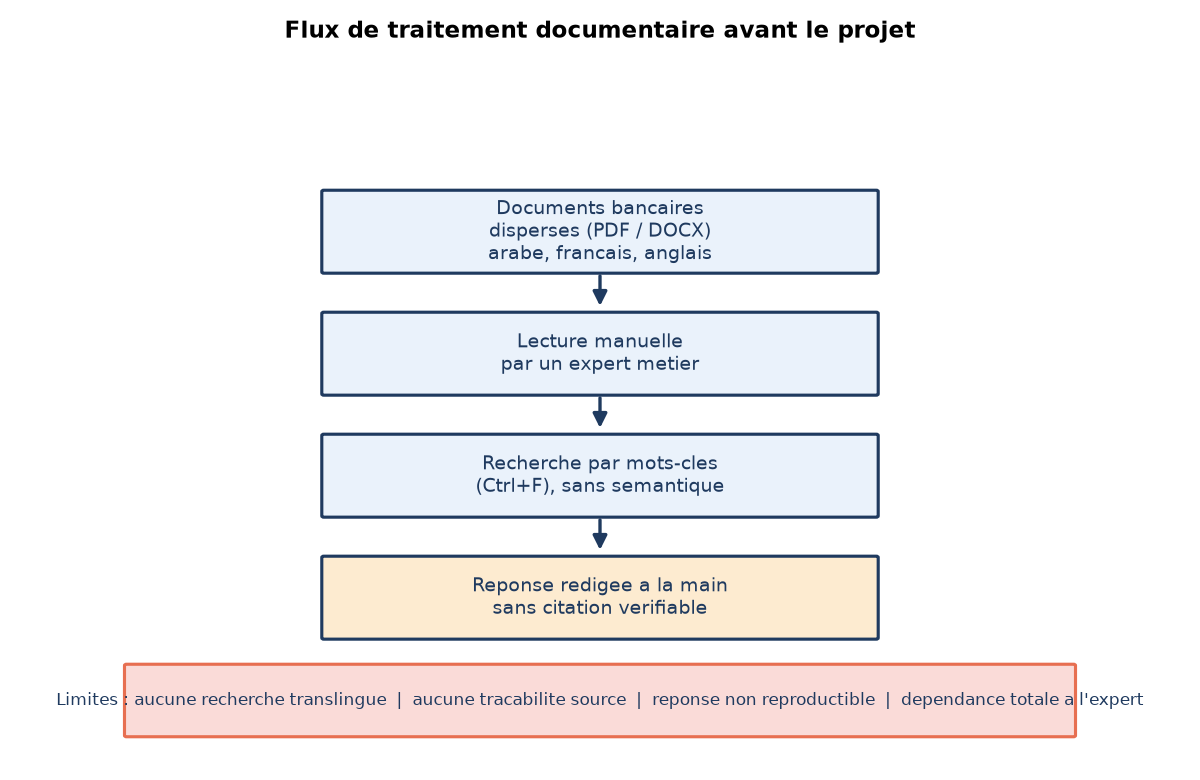
\includegraphics[width=0.8\textwidth]{workflow_before.png}
\caption{Flux documentaire avant le projet RAGLab}
\small{Interpr\'etation : ce sch\'ema illustre comment les documents \'etaient consult\'es manuellement, sans recherche s\'emantique ni tra\c{c}abilit\'e. Il permet de visualiser les limites du syst\`eme existant : d\'ependance \`a l'expert, absence de r\'eponses translingues et de citations contr\^olables.}
\end{figure}

\subsection{Journal du travail : commits de la branche}
Le travail est versionn\'e sur la branche \texttt{arena/01a0ec17-raglab}. L'historique utile se r\'esume au commit de livraison du laboratoire complet :
\begin{verbatim}
f41e557 PROD_IMAGE.md: document the no-script Windows import ...
73210f7 Initial commit
\end{verbatim}
Le commit \texttt{f41e557} concentre la totalit\'e du laboratoire : 159 fichiers, environ 66\,000 lignes ajout\'ees, dont 39 modules Python (environ 21\,300 lignes), 4 documents bancaires r\'eels d'\'evaluation, 6 jeux de questions r\'ef\'erenc\'es, 7 workflows d'int\'egration continue et une image Docker de production. C'est ce contenu, et les rapports de mesure qu'il contient, qui sert de mati\`ere premi\`ere aux chapitres 2 et 3.

\subsection{Planning pr\'evisionnel du stage}
\begin{figure}[H]
    \centering
    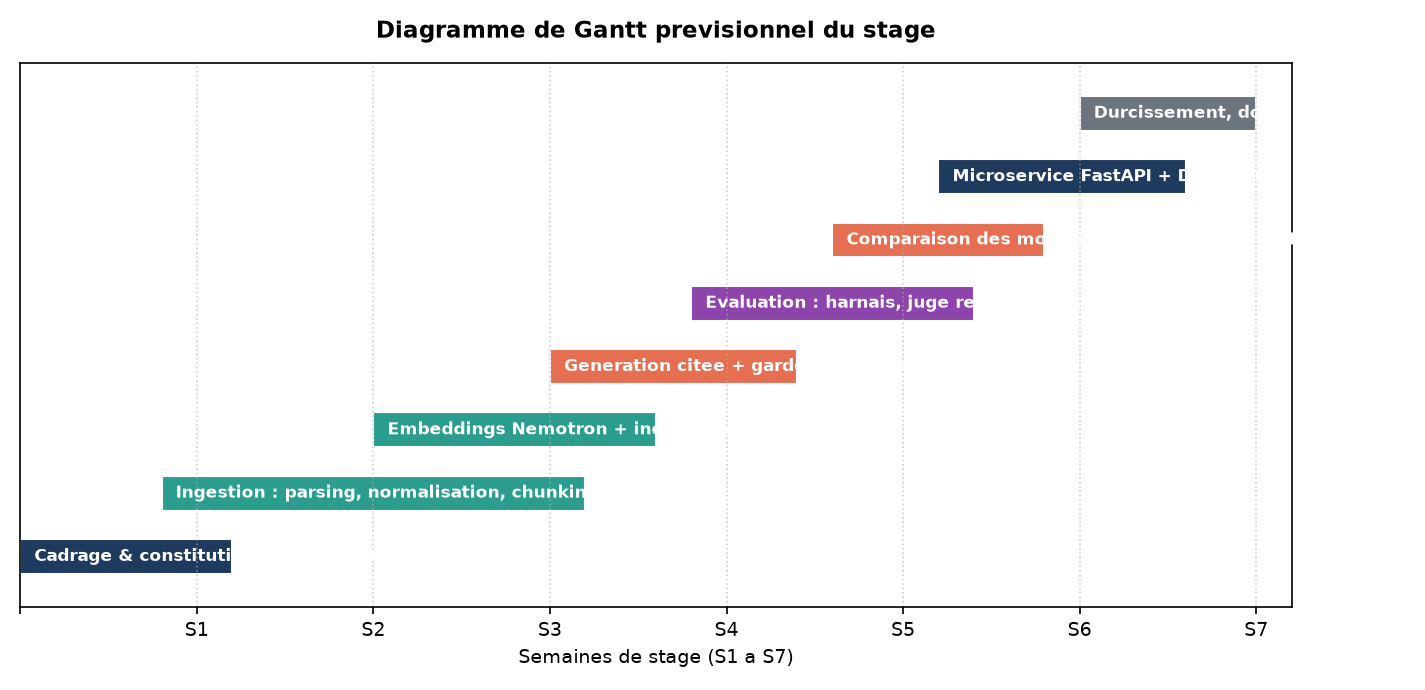
\includegraphics[width=0.95\textwidth]{gantt_stage.png}
    \caption{Diagramme de Gantt du stage (7 semaines, de S1 \`a S7)}
    \small{Interpr\'etation : ce diagramme montre la planification temporelle des activit\'es : constitution du corpus, ingestion, embeddings, g\'en\'eration cit\'ee, \'evaluation, comparaison de mod\`eles et industrialisation. Il permet de comprendre la structuration du travail, du cadrage \`a la livraison du service conteneuris\'e.}
\end{figure}

\section{M\'ethodologie adopt\'ee}
La m\'ethodologie choisie est une d\'emarche exp\'erimentale outill\'ee, adapt\'ee \`a un syst\`eme d'IA \'evalu\'e par la mesure :
\begin{enumerate}
    \item \textbf{Cadrage et corpus :} s\'election de documents bancaires r\'eels (loi, circulaire, guides) et de fiches fictives pour les essais, avec jeux de questions gel\'es par langue.
        \item \textbf{Ingestion reproductible :} parsing, normalisation arabe, d\'ecoupage versionn\'e (empreinte v4) et cache d'embeddings resumable.
    \item \textbf{Recherche contrainte et g\'en\'eration cit\'ee :} top-5 cosinus sur requ\^ete d'origine, claims JSON \`a citations mot-\`a-mot, refus en cas d'\'echec.
    \item \textbf{Mesure syst\'ematique :} harnais A/B, juge de retrieval sans LLM, comparaison de mod\`eles gratuits sur rubriques gel\'ees, CI qui rejoue les mesures.
    \item \textbf{Industrialisation :} microservice REST, image Docker portable, documentation de contrat pour les \'equipes clientes.
\end{enumerate}

\section{Conclusion}
Cette premi\`ere \'etude permet de cerner les besoins de l'entreprise, de comprendre la structure du corpus bancaire trilingue et de d\'efinir les objectifs du projet : une r\'eponse cit\'ee et refusable plut\^ot qu'une r\'eponse fluide mais inv\'erifiable, tout en identifiant les contraintes (qualit\'e du d\'ecoupage, co\^ut des appels mod\`eles, limites du gratuit).

% ======================
% CHAPITRE 2
\chapter{Conception de la solution}
\section{Introduction}
La conception repose sur la d\'efinition des besoins, l'architecture fonctionnelle et le choix du pipeline RAG. L'accent a \'et\'e mis sur la reproductibilit\'e (graines, caches, empreintes), la mesurabilit\'e (jeux gel\'es, harnais rejouables) et la s\'ecurit\'e des r\'eponses (citations exig\'ees, refus local).

\section{Environnement de d\'eveloppement}
\begin{itemize}
    \item Python 3.11, sans framework d'orchestration (ni LangChain ni LlamaIndex) et sans SDK propri\'etaire (HTTPS standard).
    \item ChromaDB persistant local (similarit\'e cosinus) + BM25 : recherche vectorielle et lexicale sans base externe.
    \item FastAPI + Uvicorn : microservice REST de 25 routes, documentation OpenAPI \`a \texttt{/docs}.
    \item tiktoken (\texttt{cl100k\_base}) et pypdf : tokenisation de r\'ef\'erence et lecture des PDF.
    \item GitHub Actions : 7 workflows (tests, images Docker, mod\`eles gratuits, hard-harness, juge retrieval, real-test, catalogues).
\end{itemize}

\subsection{Choix technologiques}
\begin{table}[H]
\centering
\begin{tabular}{|l|p{4cm}|p{5.5cm}|}
\hline
Besoin & Choix retenu & Justification \\
\hline
Embeddings & \texttt{nemotron-3-embed-1b}, natif 2048 d & Espace unique et stable ; 62,8 \% sur requ\^etes sans mot commun contre 0 \% au lexical. \\
\hline
R\'eponses & \texttt{qwen3.8-max:free} via xKiro & Meilleur score mesur\'e (13/14 dev, 18/18 held-out), gratuit\'e v\'erifi\'ee en direct. \\
\hline
Retrieval & Top-5 cosinus, requ\^ete d'origine & La traduction de requ\^ete d\'egradait le top-1 held-out. \\
\hline
Cadre logiciel & Aucun framework RAG & D\'ependances minimales, image Docker l\'eg\`ere et auditable. \\
\hline
\end{tabular}
\caption{Justification des choix technologiques}
\end{table}

\section{Besoins fonctionnels et non fonctionnels}

\subsection{Besoins fonctionnels}
\begin{itemize}
    \item Ing\'erer des documents PDF, DOCX, TXT et Markdown avec normalisation multilingue
    \item Indexer le corpus en chunks adressables, avec une collection par couple (espace d'embedding, mode de chunking)
    \item Rechercher les passages pertinents pour une question en arabe, fran\c{c}ais ou anglais, y compris translingue
    \item G\'en\'erer des r\'eponses cit\'ees ou refuser explicitement (corpus silencieux, donn\'ees priv\'ees, donn\'ees temps r\'eel)
    \item Exposer toutes les fonctions par CLI, console interactive et API REST document\'ee
\end{itemize}

\subsection{Besoins non fonctionnels}
\begin{itemize}
    \item \textbf{Tra\c{c}abilit\'e :} chaque affirmation livr\'ee porte des citations mot-\`a-mot ; un nombre non cit\'e entra\^{\i}ne un refus
    \item \textbf{Reproductibilit\'e :} tokenizer, caches, empreintes et jeux gel\'es garantissent des mesures rejouables en CI
    \item \textbf{S\'ecurit\'e :} pas de r\'eponse sur donn\'ees priv\'ees ou temps r\'eel (garde-fous locaux), masquage des cl\'es, validation des vecteurs
    \item \textbf{Portabilit\'e :} image Docker multi-stage ex\'ecutable sans clone ni pip, y compris hors-ligne apr\`es import
    \item \textbf{Maintenabilit\'e :} un noyau partag\'e par les trois frontaux, 133 contr\^oles hors-ligne, documentation de contrat
\end{itemize}

\section{Architecture fonctionnelle}

L'architecture se compose de quatre \'el\'ements principaux :

\begin{center}
\begin{tabular}{|p{3cm}|p{3cm}|p{3cm}|p{3cm}|}
\hline
\textbf{Donn\'ees en entr\'ee} & \textbf{Traitement} & \textbf{Mod\`eles} & \textbf{R\'esultats} \\
\hline
Documents bancaires ar/fr/en & Parsing, normalisation, chunking, embeddings & Nemotron (recherche) + Qwen (r\'edaction) & R\'eponses cit\'ees ou refus motiv\'es \\
\hline
\end{tabular}
\end{center}

\subsection{Description des composants}
\begin{enumerate}
    \item \textbf{Collecte :} acquisition des documents (d\'ep\^ots \texttt{data\_dirs}, t\'el\'eversement \texttt{POST /documents} avec versions et purge cibl\'ee)
    \item \textbf{Transformation :} nettoyage, r\'eparation du texte arabe, d\'ecoupage (\texttt{restructure}/\texttt{size}/\texttt{manual}) et plongements vectoriels
    \item \textbf{Application :} recherche top-5 et ex\'ecution du mod\`ele de r\'eponse derri\`ere le portillon de citations
    \item \textbf{G\'en\'eration :} production de la r\'eponse finale cit\'ee, ou d'un refus diagnostiquable avec les extraits fournis
\end{enumerate}

\section{Pipeline retenu : retrieval Nemotron + r\'eponses Qwen}
\subsection{Description et justification}
Le pipeline est gel\'e par le module \texttt{pipeline\_policy.py} : toute substitution de mod\`ele sur les chemins mesur\'es l\`eve une erreur au lieu d'un appel silencieux vers un autre mod\`ele.
\begin{table}[H]
\centering
\begin{tabular}{|l|p{8cm}|}
\hline
Param\`etre & Description \\
\hline
\texttt{embedding\_model} & \texttt{nvidia/nemotron-3-embed-1b}, natif 2048 dimensions \\
\hline
\texttt{answer\_model} & \texttt{qwen/qwen3.8-max:free} via xKiro, prompt \texttt{grounded-v1} \\
\hline
\texttt{top\_k} & 5 chunks (requ\^ete d'origine, similarit\'e cosinus) \\
\hline
\texttt{chunking} & \texttt{restructure} par d\'efaut ; 220/40, tokenizer \texttt{cl100k\_base} \\
\hline
\texttt{batch\_size} & 32 textes par appel d'embeddings, retries + bissection \\
\hline
\texttt{citation\_gate} & Citations mot-\`a-mot exig\'ees, nombres pr\'esents dans les citations \\
\hline
\texttt{free\_price\_check} & V\'erification de gratuit\'e en direct avant chaque appel Qwen \\
\hline
\end{tabular}
\caption{Param\`etres principaux du pipeline RAG}
\end{table}

\section{Diagramme de l'architecture}
\begin{figure}[H]
\centering
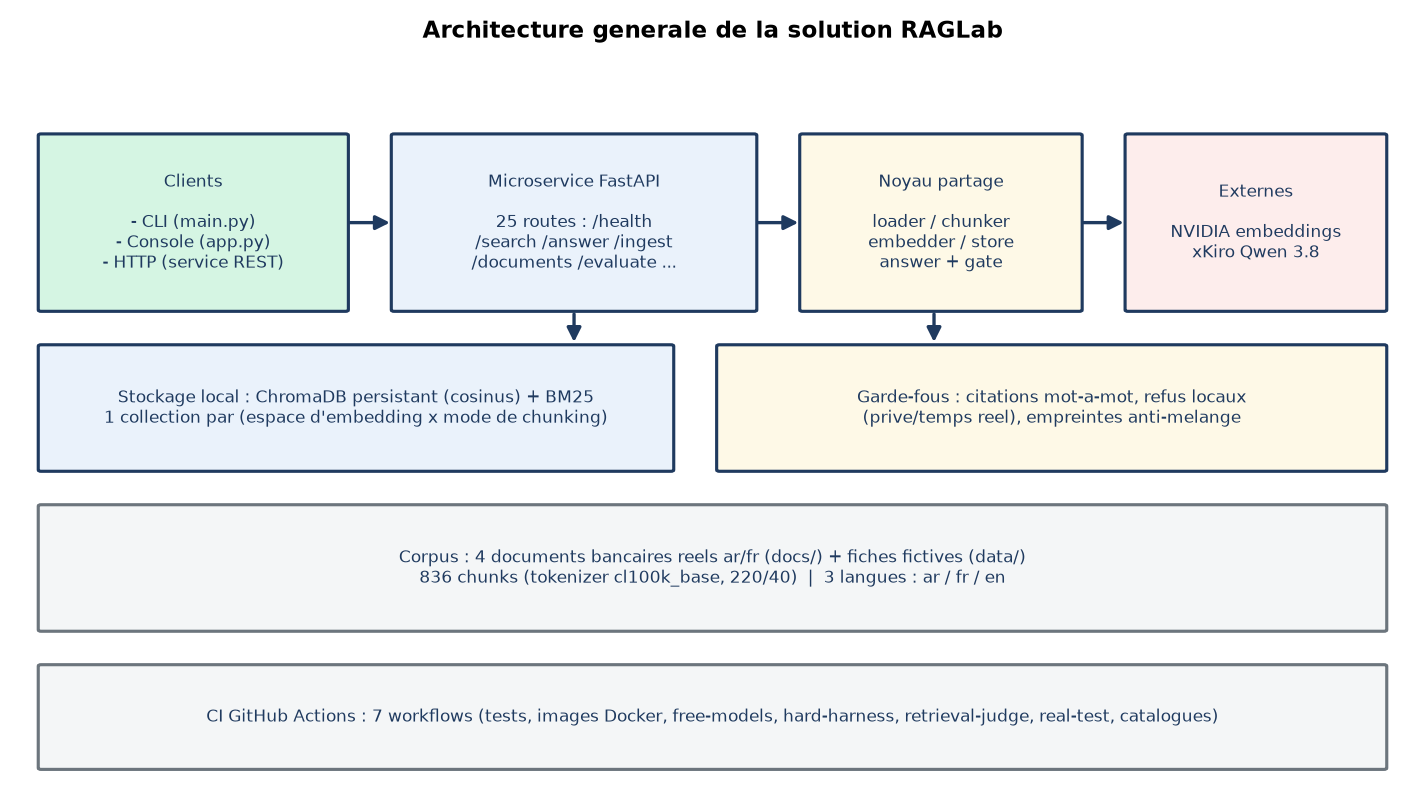
\includegraphics[width=0.95\textwidth]{architecture_diagram.png}
\caption{Architecture g\'en\'erale de la solution}
\small{Interpr\'etation : ce diagramme montre les trois frontaux partageant un m\^eme noyau, le service REST de 25 routes, le stockage et les garde-fous locaux. Il illustre comment seuls les embeddings et la r\'edaction font appel \`a des mod\`eles externes.}
\end{figure}

\subsection{Pipeline de traitement des donn\'ees}
\begin{figure}[H]
\centering
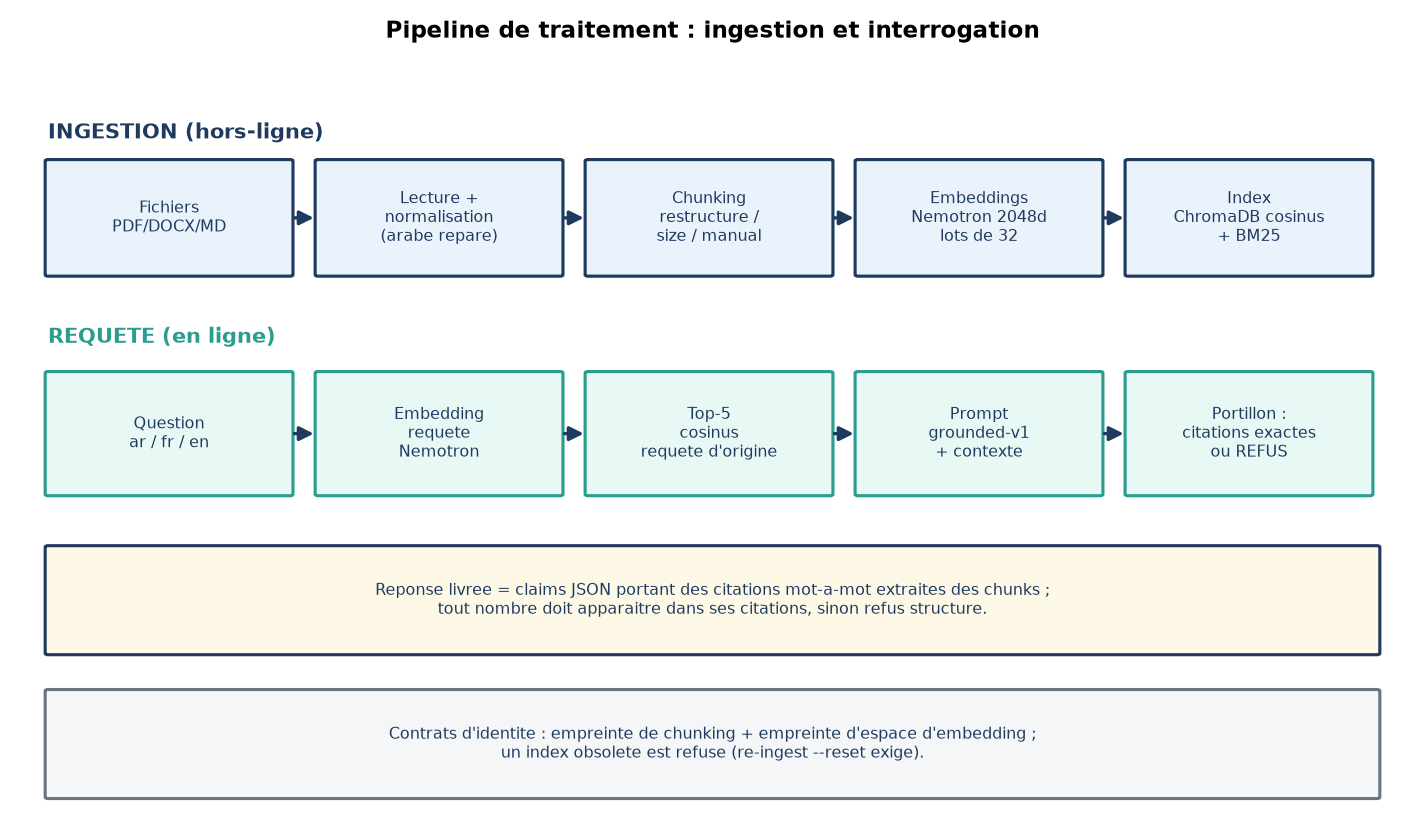
\includegraphics[width=0.95\textwidth]{data_pipeline.png}
\caption{Pipeline d'ingestion et d'interrogation}
\small{Interpr\'etation : ce sch\'ema d\'etaille l'ingestion hors-ligne (index d\'ecrit par ses empreintes) et la requ\^ete en ligne (chemin contraint vers le portillon de citations). Il permet de comprendre la transformation des documents bruts en r\'eponses cit\'ees ou en refus.}
\end{figure}

\subsection{Champs d'un chunk et m\'etadonn\'ees d'index}
\begin{table}[H]
\centering
\begin{tabular}{|l|p{8cm}|}
\hline
Champ & Description \\
\hline
\texttt{index} / \texttt{source} & Position du chunk et document d'origine (\texttt{source::chunk\_NNNN}) \\
\hline
\texttt{heading} / \texttt{language} & Titre de section et langue d\'etect\'ee (ar/fr/en) \\
\hline
\texttt{token\_count} & Taille mesur\'ee au tokenizer \texttt{cl100k\_base} \\
\hline
\texttt{chunk\_fp} & Empreinte du d\'ecoupage (mode, tailles, tokenizer) -- v4 \\
\hline
\texttt{embedding\_fp} & Empreinte de l'espace d'embeddings (mod\`ele, t\^ache, dimensions) \\
\hline
\end{tabular}
\caption{Champs index\'es pour chaque chunk}
\end{table}

\section{Conclusion}
La conception fige un pipeline \'etroit mais justifi\'e par la mesure : un seul mod\`ele d'embeddings, un seul mod\`ele de r\'eponses, une retrieval top-5 sur requ\^ete d'origine et un portillon de citations qui interdit l'affirmation non sourc\'ee.

% ======================
% CHAPITRE 3
\chapter{R\'ealisation, traitements et r\'esultats}
\section{Chargement et exploration du corpus}
\begin{verbatim}
python main.py inspect --data-dir ../docs
python main.py ingest --reset --data-dir ../docs
python main.py query "What is Murabaha?" --query-lang en
python main.py answer "What is Murabaha?" --query-lang en
\end{verbatim}

\begin{table}[H]
\centering
\begin{tabular}{|l|l|l|l|}
\hline
Document & Format & Langue & R\^ole \\
\hline
Loi\_2016-48 & PDF (36 p. au total) & arabe & Corpus r\'eel d'\'evaluation \\
\hline
Circulaire\_BCT\_2019-08 & PDF & arabe & Corpus r\'eel d'\'evaluation \\
\hline
Guide\_Interne\_Isla. & DOCX & arabe & Corpus r\'eel d'\'evaluation \\
\hline
Madkhal\_Sayrafa\_Isl. & DOCX & arabe & Corpus r\'eel d'\'evaluation \\
\hline
fiche\_produit\_atlas (fr/ar) & Markdown x2 & fran\c{c}ais, arabe & Banque fictive (essais) \\
\hline
\end{tabular}
\caption{Composition du corpus}
\end{table}

\begin{table}[H]
\centering
\begin{tabular}{|l|r|}
\hline
M\'etrique & Valeur \\
\hline
Chunks (220/40, \texttt{cl100k\_base}) & 836 \\
\hline
Pages PDF & 36 \\
\hline
Empreinte du manifeste & \texttt{807785db}... (SHA-256) \\
\hline
Couverture des preuves attendues & 16/16 (100 \%) \\
\hline
Chunks de m\'etadonn\'ees de titres & 0 \\
\hline
Dimensions d'embeddings & 2048 (natives) \\
\hline
\end{tabular}
\caption{Statistiques descriptives du corpus index\'e}
\end{table}

\section{Analyse d\'etaill\'ee et diagnostics}
\subsection{Couverture des preuves et qualit\'e du d\'ecoupage}
\begin{table}[H]
\centering
\begin{tabular}{|l|r|}
\hline
Diagnostic & R\'esultat \\
\hline
Phrases-preuves joignables dans un chunk & 16/16 -- tout est atteignable \\
\hline
Chunks parasites (titres seuls) & 0 \\
\hline
Unit\'es sources tenant dans un chunk de 220 & 5/230 (2,2 \%) -- le chunker est le plafond \\
\hline
Plafond honn\^ete du top-5 joint & 12,2 \% de tron\c{c}ons complets \\
\hline
\end{tabular}
\caption{Diagnostics de couverture (CI et juge retrieval)}
\end{table}

\subsection{Visualisation des distributions}
\begin{figure}[H]
\centering
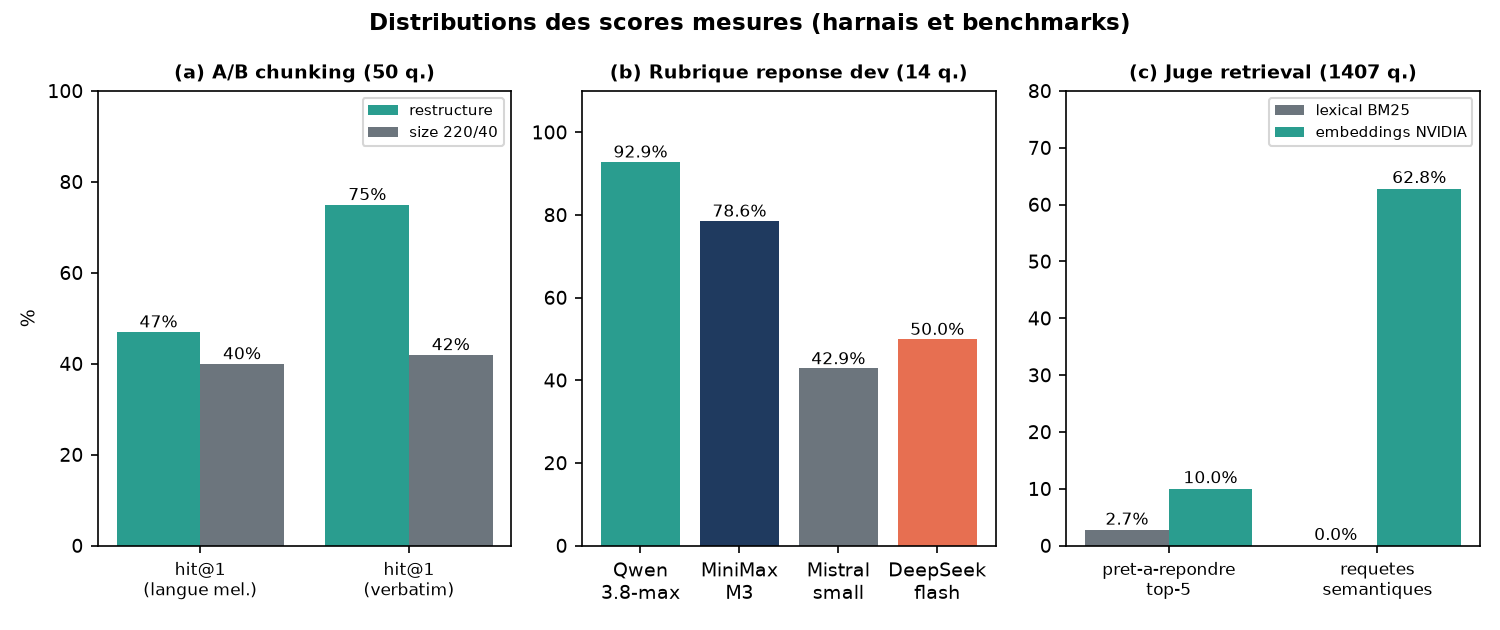
\includegraphics[width=0.95\textwidth]{score_distributions.png}
\caption{Distributions des scores mesur\'es}
\small{Interpr\'etation : (a) \texttt{restructure} bat \texttt{size} sur hit@1 global et verbatim ; (b) Qwen domine la rubrique dev ; (c) les embeddings seuls r\'esolvent les requ\^etes sans mot commun avec la preuve. Cela permet d'identifier d'un coup d'\oe il les \'ecarts entre approches.}
\end{figure}

\subsection{Matrice des m\'etriques retrieval}
\begin{figure}[H]
\centering
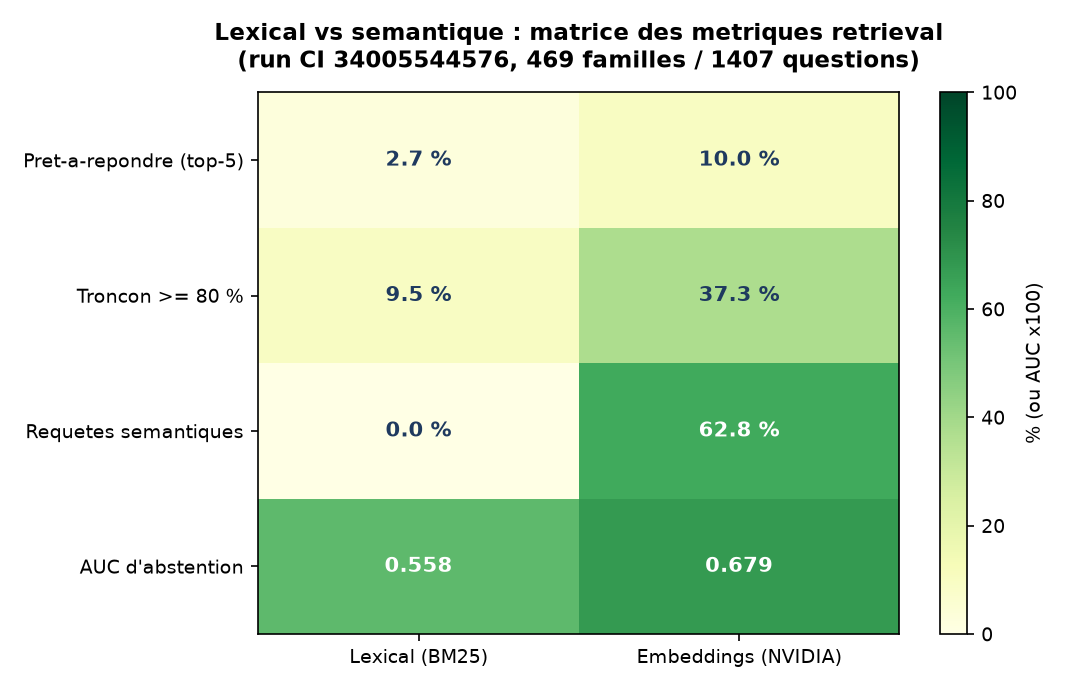
\includegraphics[width=0.8\textwidth]{metrics_heatmap.png}
\caption{Lexical contre s\'emantique : matrice des m\'etriques retrieval}
\small{Interpr\'etation : la heatmap montre que les embeddings surpassent le lexical sur les quatre axes, avec un \'ecart maximal sur les requ\^etes s\'emantiques (62,8 \% contre 0 \%). Elle aide \`a d\'ecider o\`u investir : le cross-lingue est acquis, le chunking reste le plafond.}
\end{figure}

\section{Comparaison des mod\`eles et \'evaluation}
\subsection{Banc d'essai des mod\`eles gratuits (d\'eveloppement, 16 cas)}
\begin{table}[H]
\centering
\begin{tabular}{|l|r|r|r|r|}
\hline
SKU xKiro & Rubrique & Validation & Refus & Temps moy. \\
\hline
\texttt{qwen3.8-max:free} & 13/14 (92,9 \%) & 16/16 & 2/2 & 4,68 s \\
\hline
\texttt{minimax-m3:free} & 11/14 (78,6 \%) & 15/16 & 2/2 & 6,07 s \\
\hline
\texttt{mistral-small-2603} & 6/14 (42,9 \%) & 11/16 & 2/2 & 8,27 s \\
\hline
\texttt{deepseek-v4-flash} & 7/14 (50,0 \%) & 13/16 & 2/2 & 7,46 s \\
\hline
\end{tabular}
\caption{Comparaison fra\^{\i}che des 4 candidats (5 sept. 2026)}
\end{table}

\subsection{Qwen : held-out et s\'ecurit\'e}
\begin{table}[H]
\centering
\begin{tabular}{|l|r|}
\hline
Contr\^ole & R\'esultat \\
\hline
Rubrique r\'eponses & 18/18 \\
\hline
Faux refus & 0/18 \\
\hline
Validation citations & 18/18 \\
\hline
Validation globale & 27/27 \\
\hline
Refus priv\'e/temps r\'eel & 9/9 (garde-fous locaux) \\
\hline
Injections de source & 3/3 \\
\hline
Temps client moyen & 5,25 s (18 appels) \\
\hline
\end{tabular}
\caption{Qwen held-out : 18/18 r\'eponses, 9/9 refus, 3/3 injections}
\end{table}

\subsection{A/B chunking : restructure contre fen\^etre fixe}
\begin{table}[H]
\centering
\begin{tabular}{|l|r|r|}
\hline
Mesure & \texttt{restructure} & \texttt{size} 220/40 \\
\hline
hit@1 global (50 q., BM25) & 47 \% & 40 \% \\
\hline
hit@1 verbatim & 75 \% & 42 \% \\
\hline
hit@1 mod\`eles r\'eels & 73--76 \% & 67 \% \\
\hline
Gain paraphrase / questions FR & +15 pp / +27 pp & r\'ef\'erence \\
\hline
Rappel top-20 & inf\'erieur & parfait (100 \%) \\
\hline
\end{tabular}
\caption{A/B chunking : harness50 et real-test (run 34144251576)}
\end{table}

\subsection{Juge de retrieval sans LLM (1407 questions)}
\begin{table}[H]
\centering
\begin{tabular}{|l|r|r|}
\hline
M\'etrique & Lexical (BM25) & Embeddings (NVIDIA) \\
\hline
Tron\c{c}on entier dans un chunk du top-5 & 2,7 \% & 10,0 \% \\
\hline
Tron\c{c}on \`a 80 \% & 9,5 \% & 37,3 \% \\
\hline
Requ\^etes s\'emantiques (145) & 0,0 \% & 62,8 \% \\
\hline
AUC d'abstention & 0,558 & 0,679 \\
\hline
\end{tabular}
\caption{Juge retrieval : le cross-lingue sans aucun appel g\'en\'eratif}
\end{table}

\section{Exemple de r\'eponse pour une question}
\begin{table}[H]
\centering
\begin{tabular}{|p{3.2cm}|p{6.5cm}|r|}
\hline
Question & R\'eponse du syst\`eme & Statut \\
\hline
\textit{What is Murabaha ?} (en) & 1 claim + 1 citation mot-\`a-mot ; montant repris de la citation. & Livr\'ee \\
\hline
\textit{D\'efinition du Salam ?} (fr) & 1 claim + 1 citation ; formulation valide mais hors rubrique \'etroite. & Livr\'ee \\
\hline
\textit{Solde de mon compte ?} (fr) & Refus local imm\'ediat, z\'ero appel mod\`ele (question priv\'ee). & Refus\'ee \\
\hline
\end{tabular}
\caption{Exemples illustratifs : deux r\'eponses cit\'ees, un refus local}
\end{table}

\subsection{Exemple de reclassement des strat\'egies de chunking}
\begin{table}[H]
\centering
\begin{tabular}{|l|r|r|r|r|}
\hline
Strat\'egie & Chunks & M\'ediane & Citation enti\`ere & R@1 / R@5 \\
\hline
\texttt{size} 220/40 & 310 & 186 & 45,4 \% & 47,2 \% / 70,9 \% \\
\hline
\texttt{size} 640/40 (gel\'e) & 127 & 378 & 58,7 \% & 63,8 \% / 95,0 \% \\
\hline
\texttt{size} 420/40 & 173 & 354 & 62,3 \% & 60,3 \% / 89,4 \% \\
\hline
manuelle souple & 107 & 557 & 59,0 \% & 59,2 \% / 86,2 \% \\
\hline
manuelle stricte & 211 & 153 & 59,0 \% & 55,3 \% / 83,0 \% \\
\hline
\end{tabular}
\caption{Cinq chunkings mesur\'es hors-ligne sur 282 questions}
\end{table}

\section{Grand harnais : \'etat d'avancement}
Le grand harnais vise 900 familles de questions plus 100 adversariales. Sont accept\'ees 469 familles (1\,407 paires) de cat\'egorie \textit{supported}, r\'eparties en 9 shards ; les 200 familles hors-sujet et 50 \`a preuve insuffisante restent \`a produire. L'audit crois\'e ind\'ependant est de 0/469 (second passage par le m\^eme mod\`ele). Aucun score de comparaison de r\'eponses n'est gel\'e : ce harnais est une infrastructure, pas un r\'esultat.

\section{Conclusion}
La r\'ealisation livre un laboratoire complet et mesur\'e : corpus de 836 chunks \`a couverture totale, A/B chunking gagn\'e par \texttt{restructure}, Qwen s\'electionn\'e sur banc d'essai frais puis confirm\'e en held-out (18/18), preuve cross-lingue apport\'ee sans LLM (62,8 \% contre 0 \%) et 133 contr\^oles hors-ligne au vert. Chaque chiffre est rattach\'e \`a son run, son hash git ou son JSON de preuve.

% ======================
% CHAPITRE 4
\chapter{Conclusion g\'en\'erale et perspectives}
\section*{Conclusion}
\addcontentsline{toc}{section}{Conclusion}
Le stage a permis de concevoir et d'\'evaluer un syst\`eme RAG multilingue complet pour documents bancaires : ingestion de 4 documents r\'eels en 836 chunks, indexation par embeddings natifs 2048 d, g\'en\'eration cit\'ee avec portillon de citations et refus contr\^ol\'es, le tout expos\'e en CLI, console et microservice REST conteneuris\'e. Les mesures montrent que le d\'ecoupage restructur\'e am\'eliore le hit@1 de 7 points (jusqu'\`a 9 sur mod\`eles r\'eels), que Qwen 3.8 via xKiro atteint 92,9 \% en d\'eveloppement et 100 \% en held-out, et que les embeddings r\'esolvent 62,8 \% des requ\^etes sans mot commun contre 0 \% au lexical. L'approche a aussi identifi\'e le vrai plafond du syst\`eme : le chunker, seules 5 unit\'es sources sur 230 tenant dans un chunk de 220 tokens.

\section*{Limites et Recommandations}

\begin{itemize}
    \item \textbf{Preuves \'eppill\'ees par le chunking fin} \rightarrow\ passer le d\'efaut applicatif \`a 420--640 tokens et g\'en\'eraliser l'enrichissement par voisins
    \item \textbf{Serving gratuit non garanti (quotas, routage, identit\'e du mod\`ele)} \rightarrow\ contrat fournisseur approuv\'e, capacit\'e mesur\'ee et astreinte avant production
    \item \textbf{Jeux d'\'evaluation petits et corr\'el\'es, audit non ind\'ependant (0/469)} \rightarrow\ finir les 431 familles, ajouter les 250 n\'egatives, imposer l'audit crois\'e
    \item \textbf{Pas de garantie bancaire/juridique ni de preuve de s\'ecurit\'e} \rightarrow\ revue linguistique-m\'etier, tests d'injection \'elargis, pilote supervis\'e uniquement
\end{itemize}

\section*{Perspectives}
\addcontentsline{toc}{section}{Perspectives}
Trois chantiers prolongent naturellement ce travail : l'enrichissement du contexte (voisins, seuils d'abstention calibr\'es), l'ach\`evement du grand harnais trilingue avec gels de versions, et la construction du dossier de production (fournisseur approuv\'e, revue bancaire ind\'ependante, m\'etriques de disponibilit\'e). Le laboratoire est pr\^et \`a les accueillir : chaque piste s'y exprime comme une exp\'erience mesur\'ee, compar\'ee et rejouable en CI.

\end{document}
